\documentclass{beamer}
\usepackage{beamerthemesplit}
\usepackage{wrapfig}
\usetheme{SPbGU}
\usepackage{pdfpages}
\usepackage{amsmath}
\usepackage{mathtools}
\usepackage{cmap}
\usepackage{indentfirst}
\usepackage{amsmath}
\usepackage{tikz}
\usepackage{multirow}
\usepackage[noend]{algpseudocode}
\usepackage{algorithm}
\usepackage{algorithmicx}
\usepackage{ stmaryrd }
\usepackage{fancyvrb}
\usepackage{qtree}
\usepackage{verbatim}
\usepackage{ulem}
\usepackage{proof}
\usepackage{mathtools}
\usepackage{ulem}

\beamertemplatenavigationsymbolsempty

\setbeamertemplate{itemize item}[circle]
\setbeamertemplate{enumerate item}[circle]
\newcommand{\derives}[1][*]{\xRightarrow[]{#1}}

\def\To{\derives[]}
\def\iff{\Leftrightarrow}

\usetikzlibrary{shapes,arrows}
\usetikzlibrary{positioning,automata}
\tikzset{every state/.style={minimum size=0.2cm},
initial text={}
}

\graphicspath{
  {pics/}
}

\newcommand{\incimage}[2][0.8]{
  \begin{center}
    \includegraphics[width=\textwidth, height=#1\textheight, keepaspectratio]{#2}
  \end{center}
  }

\title[]{Tupling via Constructive Algorithmics}
\subtitle[]{}
\institute[]{JetBrains Programming Languages and Tools Lab
}

\author[]{Kate Verbitskaia}

\date{20.09.2021}

\definecolor{orange}{RGB}{179,36,31}

\begin{document}
{
  \begin{frame}
    \titlepage
  \end{frame}
}


\begin{frame}[fragile]
  \frametitle{What is Tupling}
\begin{center}
  Program transformation technique which groups functions \\ with same arguments together
\end{center}

\vspace{1cm}

Objectives:
\begin{itemize}
  \item Eliminate multiple traversals of the same data structure
  \item Eliminate redundant recursive calls
\end{itemize}
\end{frame}

\begin{frame}[fragile]
  \frametitle{Example: Maximum and Length}
\begin{center}
  Compute both maximum value of the list and its length
\end{center}
\end{frame}

\begin{frame}[fragile]
  \frametitle{Example: Average of the List}
\begin{center}
  Compute the average of the list of numbers
\end{center}
\end{frame}

\begin{frame}[t]
  \frametitle{Tupling via Fold/Unfold}
\textit{A Transformation System for Developing Recursive Programs.} \\R.M. Burstall and John Darlington. (1977)

\vspace{0.6cm}

Objective: Transform a ``very simple, lucid and hopefully correct program'' into a more efficient one

\vspace{0.6cm}
How: using a combination of the following transformations\footnote{And some eureka tuples}
\begin{itemize}
  \item Definition
  \item Instantiation
  \item Unfolding
  \item Folding
  \item Abstraction
  \item Laws
\end{itemize}
\end{frame}

\begin{frame}[fragile]
  \frametitle{Transformations in the Fold/Unfold Framework}
\texttt{fib 0 = 1}

\texttt{fib 1 = 1}

\texttt{fib (n+2) = fib (n+1) + fib n}

\begin{itemize}
  \item Definition
  \begin{itemize}
    \item Introduce a new recursive equation
    \item LHS should not be an instance of any other equation
    \item \texttt{g n = (fib (n+1), fib n)}
  \end{itemize}
  \item Instantiation
  \begin{itemize}
    \item Introduce a substitution instance of an existing equation
    \item \texttt{g 0 = (fib (0+1), fib 0)}
  \end{itemize}
  \item Unfolding
  \begin{itemize}
    \item Replace LHS of an equation with the corresponding instance of its RHS within some other expression
    \item \texttt{g 0 = (fib (0+1), fib 0) = (fib 1, fib 0) = (1, 1)}
  \end{itemize}

\end{itemize}
\end{frame}

\begin{frame}[fragile]
  \frametitle{Transformations in the Fold/Unfold Framework}
\begin{itemize}
  \item Abstraction
  \begin{itemize}
    \item Add a \texttt{\underline{where}} clause
    \item \texttt{g (n+1) = (fib (n+2), fib (n+1)) }
    \item \texttt{g (n+1) = (fib (n+1) + fib (n), fib (n+1))}
    \item \texttt{g (n+1) = (u + v, u) \underline{where} (u, v) = (fib (n+1), fib n)}
  \end{itemize}
  \item Folding
  \begin{itemize}
    \item Replace RHS of some equation with the instance of the LHS
    \item \texttt{g (n+1) = (u + v, u) \underline{where} (u, v) = (fib (n+1), fib n)}
    \item \texttt{g (n+1) = (u + v, u) \underline{where} (u, v) = g n}
  \end{itemize}
  \item Laws
  \begin{itemize}
    \item Rewrite equations using some laws valid in the domain
    \item \texttt{0 + 1 = 1}
    \item \texttt{x + y = y + x}
    \item \texttt{(x + y) * z = x * z + y * z}
  \end{itemize}
\end{itemize}
\end{frame}

\begin{frame}[t]
  \frametitle{Eureka Tuples}
\texttt{fib 0 = 1}

\texttt{fib 1 = 1}

\texttt{fib (n+2) = fib (n+1) + fib n}

\pause

\vspace{0.5cm}

\texttt{g n = (fib (n+1), fib n)} --- Eureka tuple

\pause

\vspace{0.5cm}

\textit{A few transformations later...}

\vspace{0.5cm}

\texttt{g 0 = (1, 1)}

\texttt{g (n+1) = (u + v, u) \underline{where} (u, v) = g n}

\vspace{0.5cm}
\texttt{fib 0 = 1}

\texttt{fib 1 = 1}

\texttt{fib (n+2) = u + v \underline{where} (u, v) = g n)}
\end{frame}

\begin{frame}[t]
  \frametitle{Tupling Strategy}
\textit{A Powerful Strategy for Deriving Efficient Programs by Transformations.} \\Alberto Pettorossi. (1984)

\vspace{0.6cm}

Objective: find a way to derive eureka steps

\vspace{0.6cm}

How: find a \textit{progressive sequence of cuts} in a dependency graph of a function with the \textit{same number} of nodes and make a tuple out of it.
\end{frame}

\begin{frame}[fragile]
  \frametitle{Progressive Sequence of Cuts}
\textit{Cut}: set of nodes in a dependency graph, s.t. if we remove them along with their edges, we are left with 2 disconnected graphs $g_1$ and $g_2$, and $\forall m$ --- node in $g_1$, $\forall n$ --- node in $g_2$: $m > n$ \footnote{$>$ is an ancestor-descendent relation}

\vspace{0.6cm}

\textit{Progressive sequence of cuts}:
\\ $\{c_i \mid 0 \le i \le k\}$,
\\ $\forall i. \ c_i \cap c_{i-1} \neq c_i \neq c_{i-1}$,
\\ $\forall m \in c_i \setminus (c_i \cap c_{i-1}). \ \exists n \in c_{i-1}. \ m > n$, and
\\ $\forall n \in c_{i-1} \setminus (c_i \cap c_{i-1} \ \exists m \in c_i. \ m > n)$
\end{frame}

\begin{frame}[fragile]
  \frametitle{Progressive Sequence of Cuts: Example}
  \begin{verbatim}
f n a b c =
  if n == 0
  then skip
  else f (n-1) a c b ++ ab ++ f (n-1) c b a
  \end{verbatim}
\begin{center}
  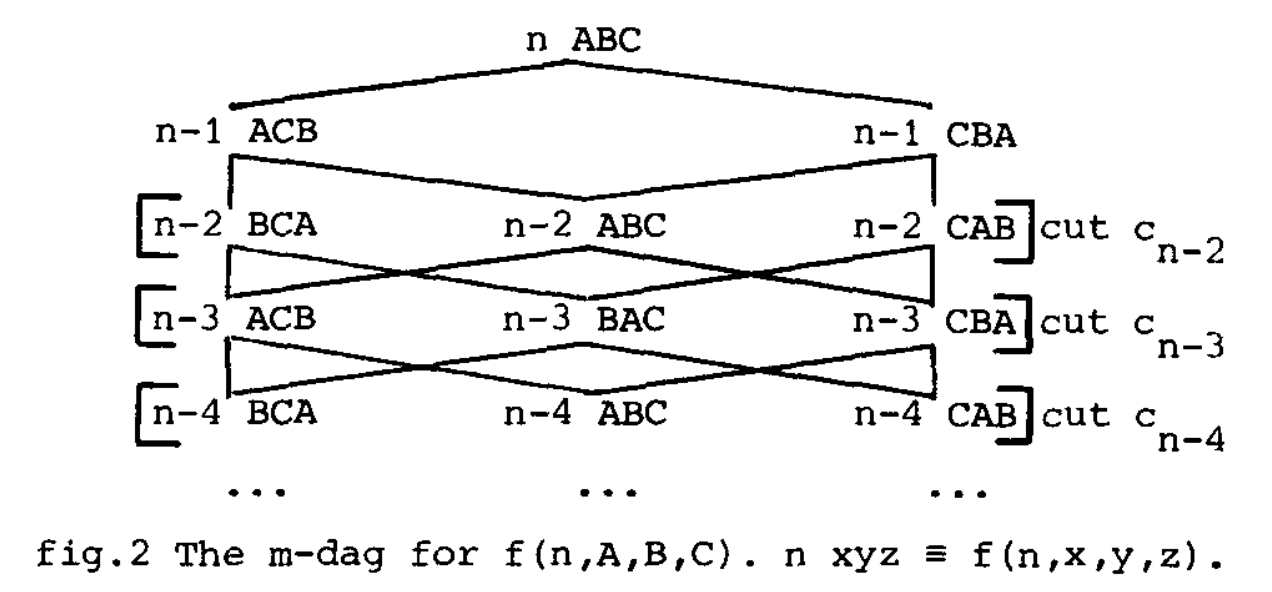
\includegraphics[width=\textwidth]{Hanoi.png}
\end{center}
\end{frame}

\begin{frame}[fragile]
  \frametitle{Tupling Strategy: Limitations}
\begin{itemize}
  \item Not fully automatic
  \item Possible heuristic 1: search for repeated computations while building dependency graph
  \item Possible heuristic 2: not unfold those recursive calls which can be derived in constant time from calls already in the cut
\end{itemize}
\end{frame}

\begin{frame}[t]
  \frametitle{Mechanizing Tupling Further}
\textit{Towards an Automated Tupling Strategy.} \\Wei-Ngan Chin. (1993)

\vspace{0.6cm}

Objective: develop a fully automatic tupling algorithm

\vspace{0.6cm}

How:
\begin{itemize}
  \item Remove the most senior nodes in a cut and replace them with their children
  \item Check if there are ancestors which match the cut
  \item If they match, it is a candidate for tupling
  \item If they do not, check the next cut
\end{itemize}
\end{frame}

\begin{frame}[fragile]
  \frametitle{Towards an Automated Tupling Strategy: Limitations}
\begin{itemize}
  \item Extension of the method:
  \begin{itemize}
    \item Tree of cuts instead of sequences
    \item Recursion parameter ordering
  \end{itemize}
  \item Termination is only guaranteed if:
  \begin{itemize}
    \item There is a single recursive parameter
    \item The recursive parameter is strictly decreasing
    \item No other parameters are accumulating
    \item All variables in recursive calls are taken from the recursive parameters
  \end{itemize}
  \item Good news: sometimes preprocessing can be used to transform the function into this form
  \item Still: Needs a clever control to avoid infinite unfolding and is not easy to implement in a real compiler
\end{itemize}
\end{frame}

\begin{frame}[t]
  \frametitle{Tupling via Constructive Algorithmics}
\textit{Tupling Calculation Eliminates Multiple Data Traversals.} \\Z. Hu, H. Iwasaki, M. Takeichi, A. Takano. (1997)

\vspace{0.6cm}

Objective: create a fully automatic tupling algorithm suitable to be used in a real compiler

\vspace{0.6cm}

How: \sout{throw some category theory at the problem}

\pause

\vspace{0.6cm}

How: use Constructive Algorithmics and Mutu theorem
\end{frame}

\begin{frame}[fragile]
  \frametitle{Constructive Algorithmics}
  \begin{itemize}
    \item Represent data types as \textit{polynomial endofunctors}
    \item Represent recursive functions as \textit{catamorphisms}
    \item Use \textit{Mutu theorem} and other \textit{laws} to transform recursive functions
  \end{itemize}
\end{frame}

\begin{frame}[fragile]
  \frametitle{Constructive Algorithmics: Polynomial Endofunctors}
\begin{itemize}
  \item Identity
  \begin{itemize}
    \item $I \ X = X$
    \item $I \ f = f$
  \end{itemize}
  \item Constant
  \begin{itemize}
    \item $!A \ X = A$
    \item $!A \ f = id$
  \end{itemize}
  \item Product $X \times Y$
  \begin{itemize}
    \item $X \times Y = \{(x, y) \mid x \in X, y \in Y\}$
    \item $\pi_1 (a, b) = a$
    \item $\pi_2 (a, b) = b$
    \item $(f \times g) (x, y) = (f \ x, g \ y)$
    \item $(f \triangle g) a = (f \ a, g \ a)$
  \end{itemize}
  \item Separated sum $X + Y$
  \begin{itemize}
    \item $X + Y = \{1\} \times X \cup \{2\} \times Y$
    \item $(f + g) (1, x) = (1, f \ x)$
    \item $(f + g) (2, y) = (2, g \ y)$
    \item $(f \triangledown g) (1, x) = f \ x $
    \item $(f \triangledown g) (2, y) = g \ y $
  \end{itemize}
\end{itemize}
\end{frame}

\begin{frame}[fragile]
  \frametitle{Polynomial Functors: List}

\texttt{data List a = Nil | Cons a (List a)}

\vspace{0.5cm}

$F_{L_A} = !1 + !A \times I$

\vspace{0.5cm}

$in_{F_{L_A}} = Nil \triangledown Cons$

\vspace{0.5cm}

\begin{verbatim}
out = \xs . case xs of
              Nil -> (1, ())
              Cons a as -> (2, (a, as))
\end{verbatim}

\end{frame}

\begin{frame}[fragile]
  \frametitle{Polynomial Functors: Binary Tree}
\texttt{data Tree a = Leaf a | Node (Tree a) (Tree a)}

\vspace{0.5cm}

$F_{T_A} = !A + I \times I$

\vspace{0.5cm}

$in_{F_{T_A}} = Leaf \triangledown Node$

\vspace{0.5cm}

\begin{verbatim}
out = \t . case t of
             Leaf a -> (1, a)
             Node l r -> (2, (l, r))
\end{verbatim}

\end{frame}

\begin{frame}[fragile]
  \frametitle{Catamorphisms: List}

\begin{verbatim}
cata [] = e
cata (x : xs) = x + (cata xs)
\end{verbatim}

Here \texttt{e} and \texttt{+} uniquely determine a catamorphism over lists

\vspace{0.3cm}

Can be rewritten: $cata = ([e \triangledown +])_{F_{L_A}}$

\vspace{0.3cm}

Catamorphisms over a data type captured by functor $F$ is characterized by:

$$
h = ([\phi])_F \ \equiv \ h \, \circ \, in_F = \phi \, \circ \, F \, h
$$
\end{frame}


\begin{frame}[fragile]
  \frametitle{Catamorphisms: List Sum}
$$sum = ([0 \triangledown plus])$$

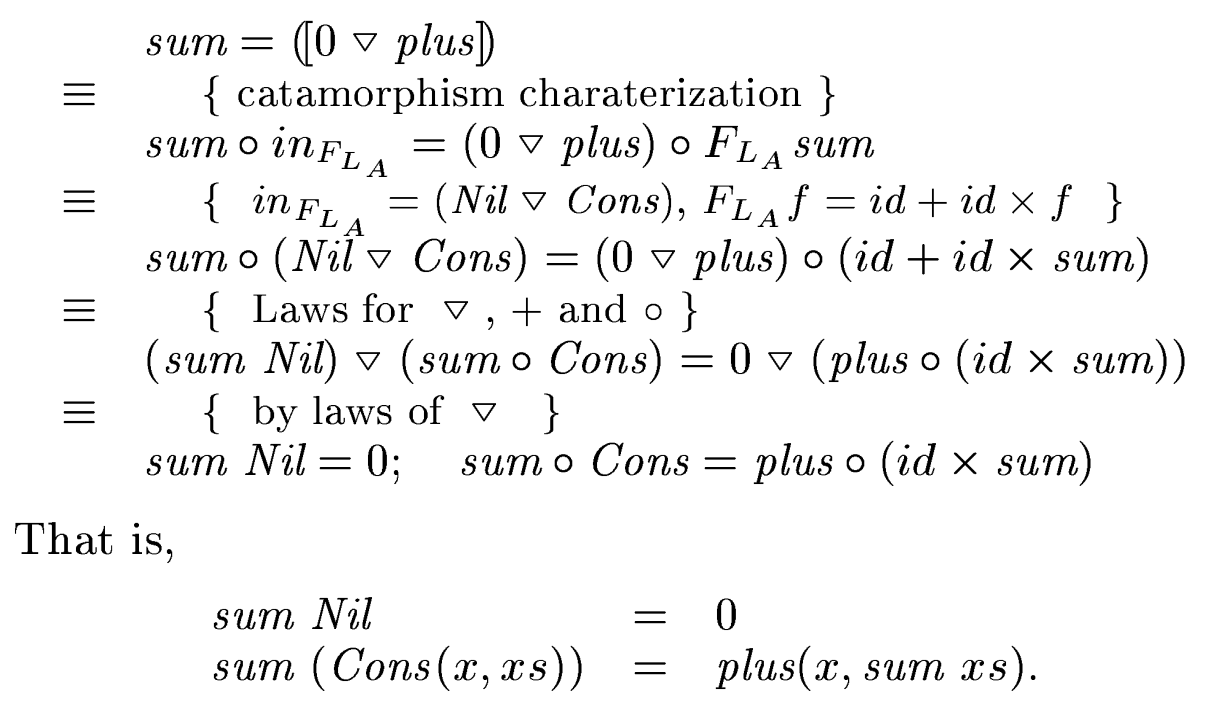
\includegraphics[width=\textwidth]{sum.png}
\end{frame}

\begin{frame}[fragile]
  \frametitle{The Mutu Tupling Theorem}
\begin{center}
  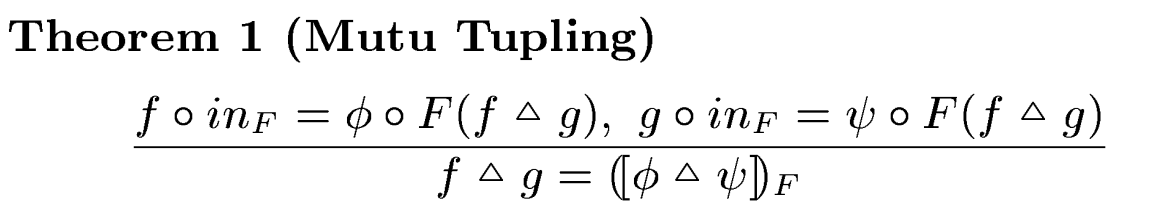
\includegraphics[width=\textwidth]{mutu.png}
\end{center}

\begin{itemize}
  \item Functions which traverse over the same data structure (in a specific regular way) should be tupled
  \item Tupling should be done with a catamorphism
\end{itemize}
\end{frame}

\begin{frame}[fragile]
  \frametitle{Example: Deepest Leaves}
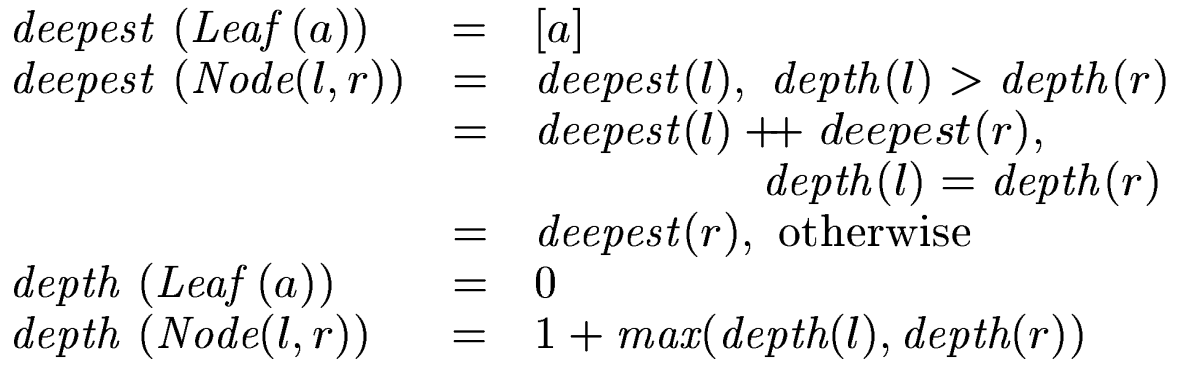
\includegraphics[width=\textwidth]{deepestOrig.png}
\end{frame}

\begin{frame}[fragile]
  \frametitle{Deepest Leaves: Mutu Theorem Application}
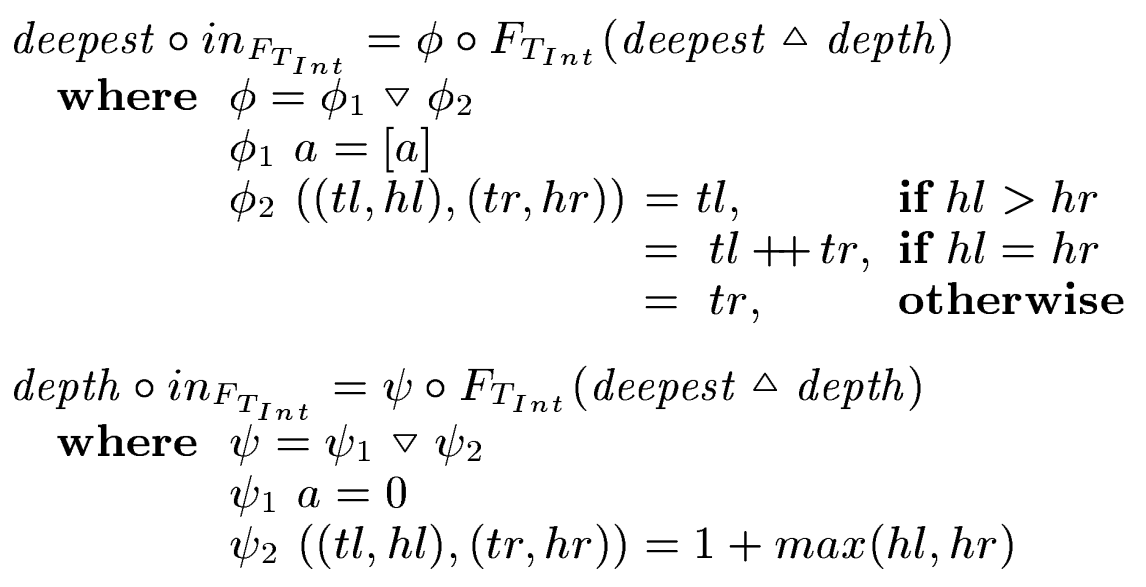
\includegraphics[width=\textwidth]{deepestMutu.png}

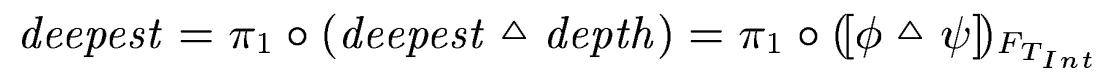
\includegraphics[width=\textwidth]{deepestDef.png}
\end{frame}

\begin{frame}[fragile]
  \frametitle{Main Property of the Approach}
\begin{center}
  All multiple data traversals by tuplable functions in a program can be eliminated by tuple calculation
\end{center}
\end{frame}

\begin{frame}[fragile]
  \frametitle{Multiple Data Traversal}
\textit{Multiple data traversal}: if there exists two calls $f \ p$ and $f' \ p'$, in which $p$ is equal or is a sub-pattern of $p'$
\end{frame}

\begin{frame}[fragile]
  \frametitle{Tuplable Functions}
Mutually recursive functions:
$$f_1, \dots, f_m$$

Defined by equations:
$$f_i \ p_{ij} \ v_{s_1} \dots v_{s_{n_i}} = e_{ij}$$

\vspace{0.3cm}

$f_1, \dots, f_m$ are called \textit{tuplable} if for every occurance of recursive calls to $f_1, \dots, f_m$ in all $e_{ij}$, say $f_k \ e' \ e_1 \dots e_{n_k}$, $e'$ is a sub-pattern of $p_{ij}$
\end{frame}

\begin{frame}[fragile]
  \frametitle{Tuplable Functions: Examples}
Example:

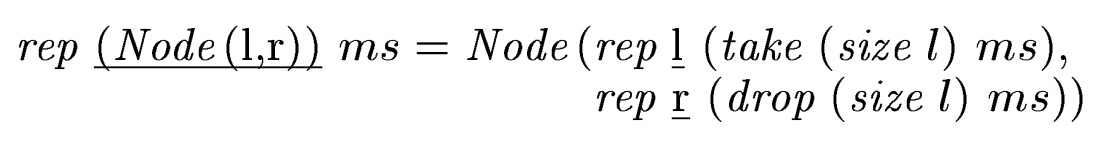
\includegraphics[width=\textwidth]{tupExample.png}

\vspace{0.6cm}

Non-Example:

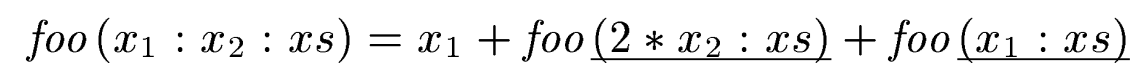
\includegraphics[width=\textwidth]{tupNonExample.png}
\end{frame}

\begin{frame}[fragile]
  \frametitle{Standardizing}
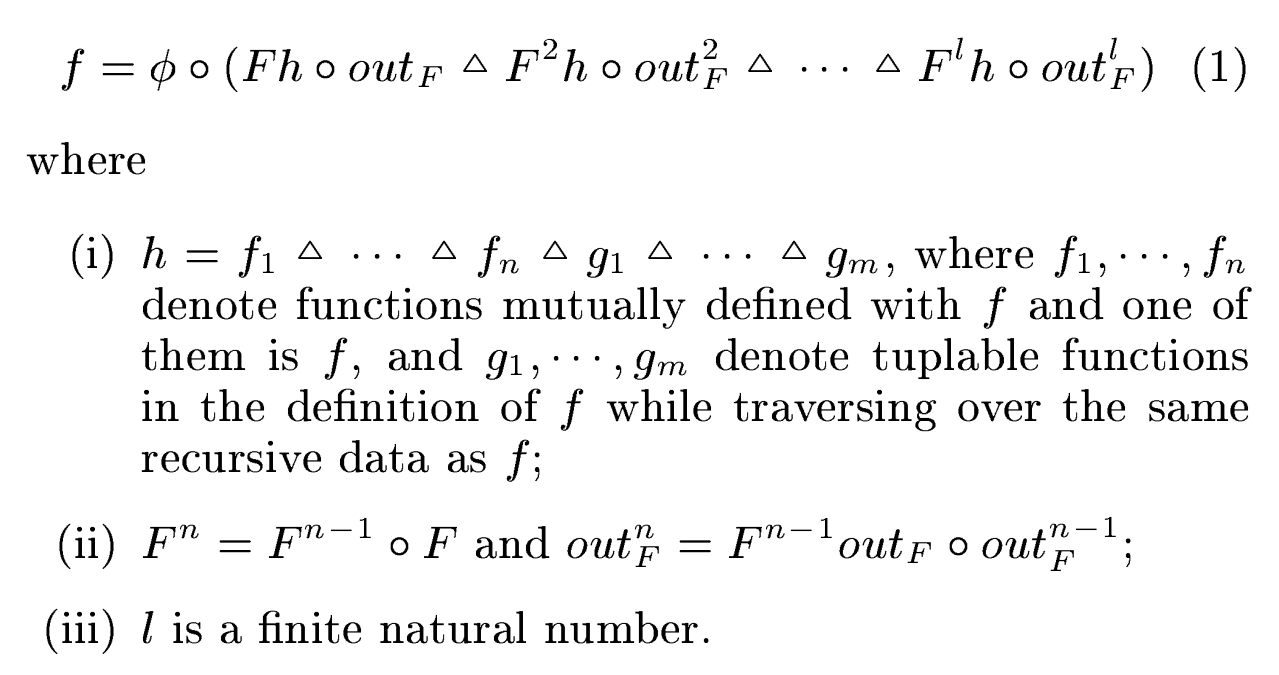
\includegraphics[width=\textwidth]{standard.png}
\end{frame}

\begin{frame}[fragile]
  \frametitle{Manipulation of Functions in Standard Form}
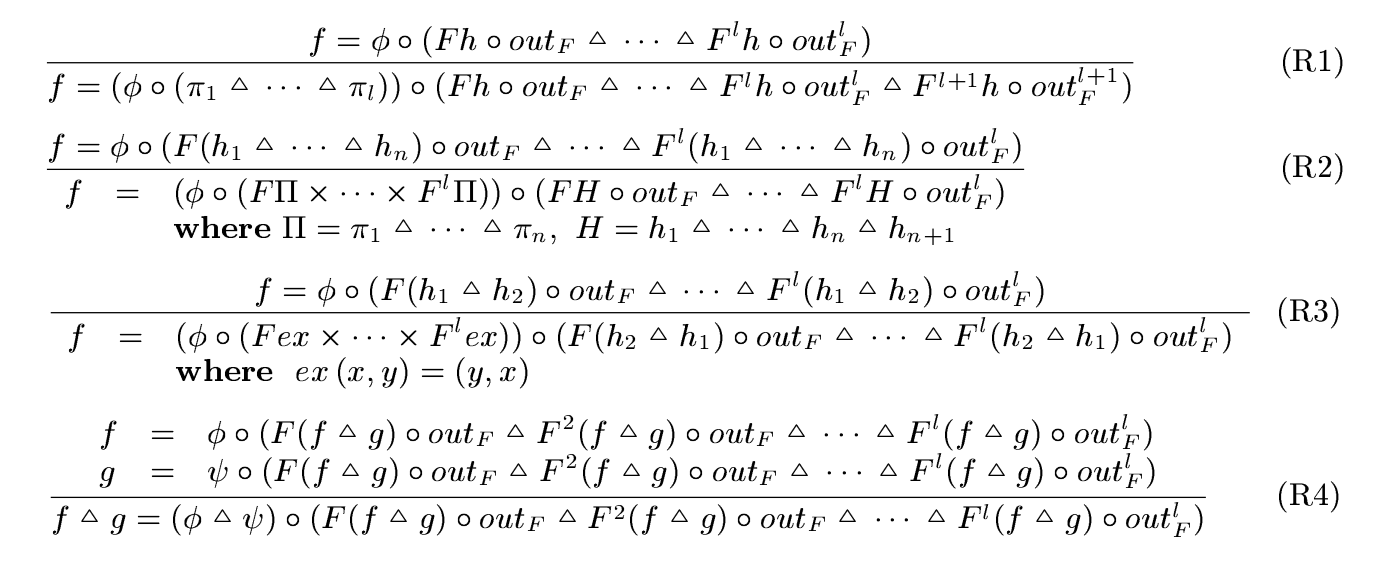
\includegraphics[width=\textwidth]{manipulation.png}
\end{frame}

\begin{frame}[fragile]
  \frametitle{Tupling of Tuplable Functions}
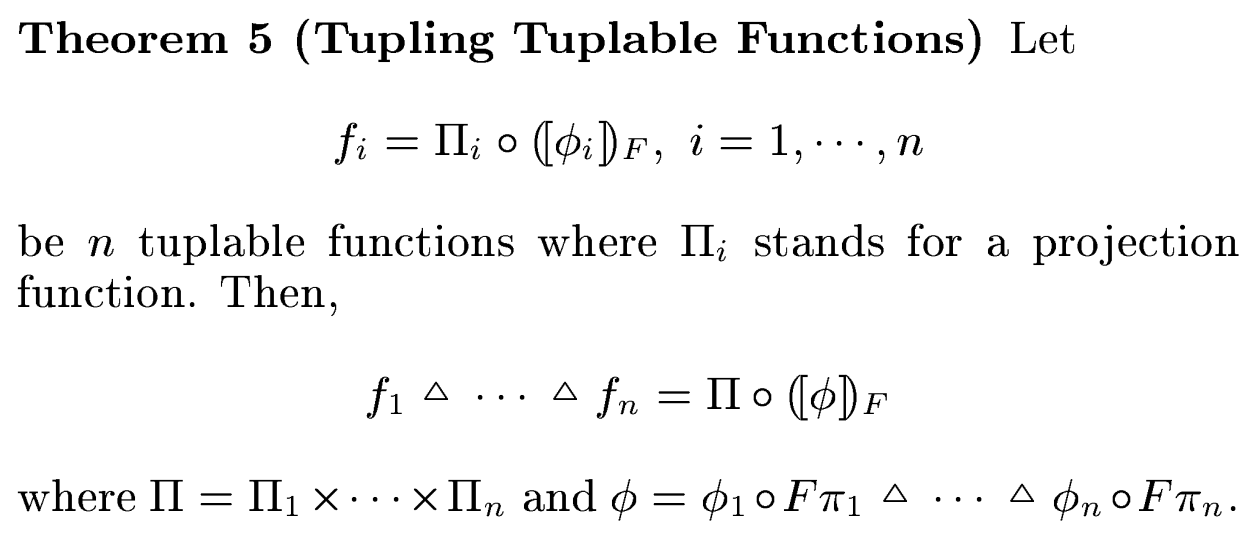
\includegraphics[width=\textwidth]{tupling.png}
\end{frame}

\begin{frame}[fragile]
  \frametitle{Example: Fibonacci}
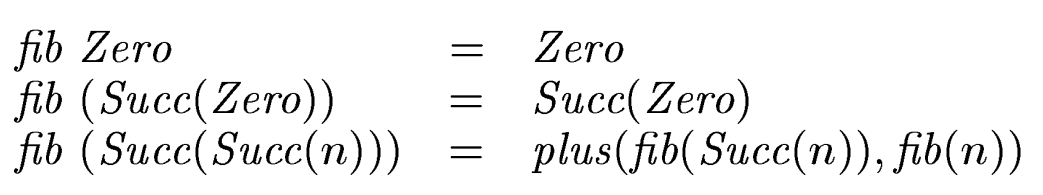
\includegraphics[width=0.9\textwidth]{fibDef.png}

\vspace{0.3cm}

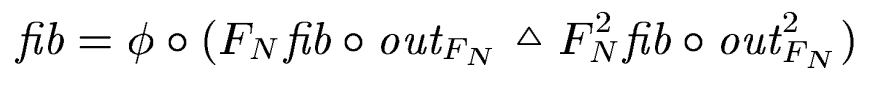
\includegraphics[width=0.6\textwidth]{fibDef1.png}

\vspace{0.3cm}

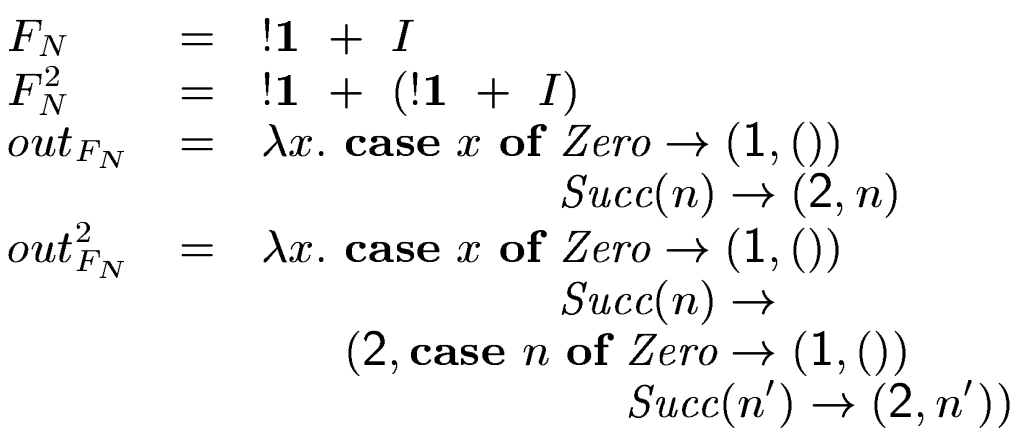
\includegraphics[width=0.7\textwidth]{Nat.png}
\end{frame}

\begin{frame}[fragile]
  \frametitle{Example: Fibonacci}
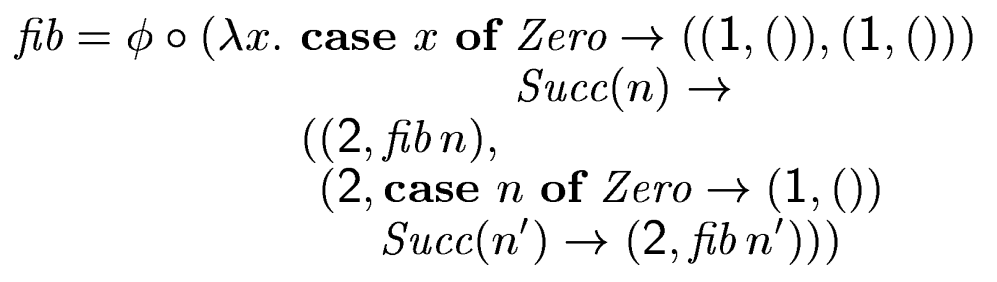
\includegraphics[width=0.5\textwidth]{fibPhi.png}

\vspace{0.3cm}

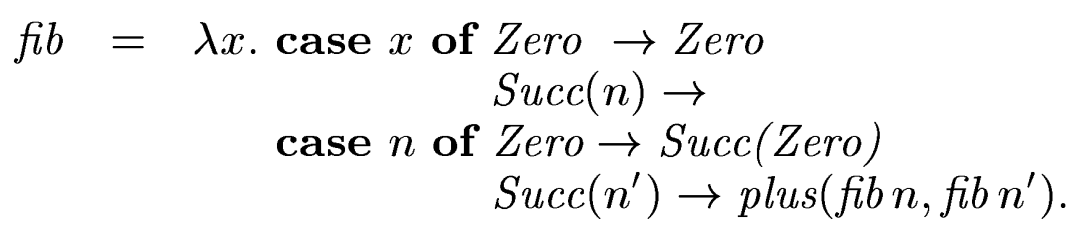
\includegraphics[width=0.55\textwidth]{fibRed.png}

\vspace{0.3cm}

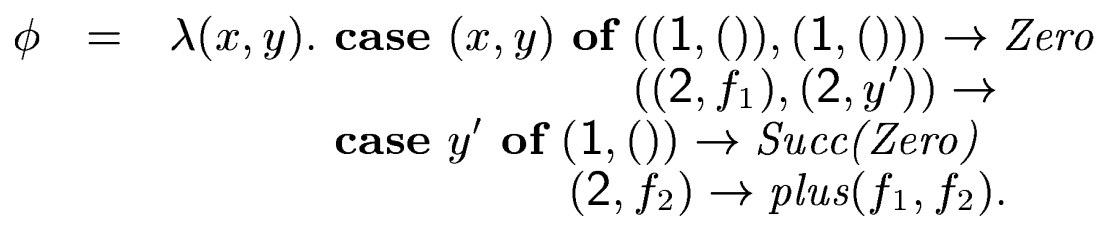
\includegraphics[width=0.55\textwidth]{phi.png}

\vspace{0.3cm}

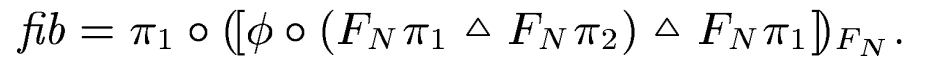
\includegraphics[width=0.4\textwidth]{fibFinal.png}
\end{frame}

\begin{frame}[fragile]
  \frametitle{Fibonacci: Result}
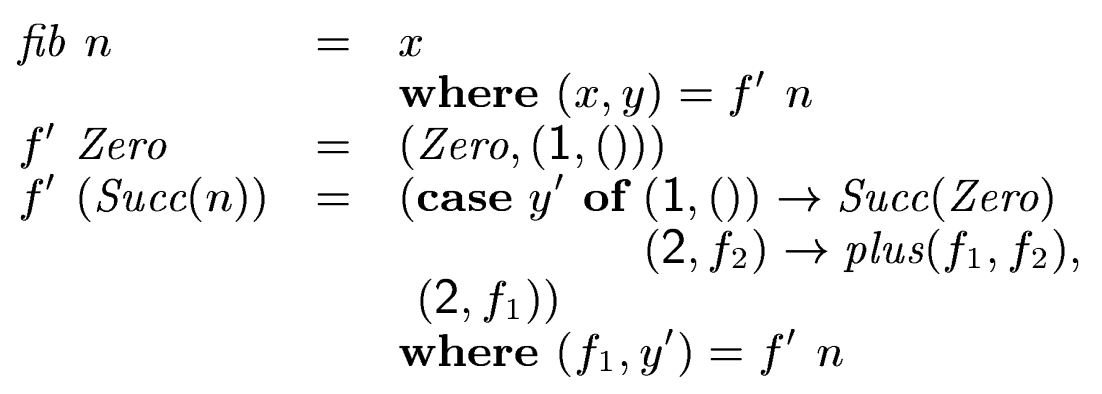
\includegraphics[width=0.8\textwidth]{fibResult.png}
\end{frame}

\begin{frame}[fragile]
  \frametitle{Tupling Calculation: Properies and Limitations}
\begin{itemize}
  \item[+] The algorithm is correct
  \item[+] The algorithm terminates
  \item[+] All multiple data traversals by tuplable functions can be eliminated
  \item[--] Tupled functions require extra memory
  \item[--] Needs an efficient tuple implementation
\end{itemize}
\end{frame}

\begin{frame}[fragile]
  \frametitle{Literature}
\begin{itemize}
  \item \textit{A Transformation System for Developing Recursive Programs.} \\ R.M. Burstall and John Darlington. (1977)
  \item \textit{A Powerful Strategy for Deriving Efficient Programs by Transformations.} Alberto Pettorossi. (1984)
  \item \textit{Towards an Automated Tupling Strategy.} Wei-Ngan Chin. (1993)
  \item \textit{Tupling Calculation Eliminates Multiple Data Traversals.} \\Z. Hu, H. Iwasaki, M. Takeichi, A. Takano. (1997)
\end{itemize}
\end{frame}
\end{document}